

\chapter{提取特征}
\label{chap:feature}
本文采用的是基于特征的方法,如何用合适的特征描述图像显得至关重要。首先,选取的特征需要能很好地刻画人物的姿态信息,即相似姿态具有相似的特征,不同姿态的特征的区别也要足够明显,尽可能让特征只包含姿态信息,不会因为光照、图片尺寸、衣服、人物体型的改变受到剧烈变化。其次,特征的维数不能太高,否则会增加学习和预测过程中的计算量。同时提取特征本身的计算量也要加以限制。
经过调查发现,目前最好的姿态估计算法~\cite{ramanan2007learning}~\cite{yang2011articulated}~\cite{tian2012exploring} 大都采用了HOG(Histogram of Oriented Gradient,梯度直方图)的特征,也有一些文献采用了其他的特征,如\cite{bo2008fast}采用了SIFT和HistoSC的特征,\cite{eth_biwi_01027}采用了Lab颜色空间统计和皮肤检测的特征,本文同多数算法一样采用了HOG 特征,并做了一些改进,此外,还提出了一种能表示皮肤信息的特征,取得了较好的结果。
\section{图片预处理}
为了剔除环境对提取特征的影响,在提取特征前首先要提取ROI(Region Of Interests)。在本文中,ROI即为图片中的人物,提取ROI即背景分离,任务是把人物从图片中分割出来,并裁剪图片。由图\ref{fig:demo}可以看出HumanEva数据库的环境是非常复杂的,好在数据库提供了纯背景的图像序列\ref{fig:background},因此可以在已知背景情况下分割人物。尽管这项任务是计算机视觉领域中一个非常久远且已经攻克的问题,但由于这不是本文重点,因此没有花太多时间和精力调查文献和实现算法,用一系列简单的操作实现了比\cite{Poppe2007}更好的分割效果。
\begin{figure}[htbp]
  \centering
  \subcaptionbox{C1}{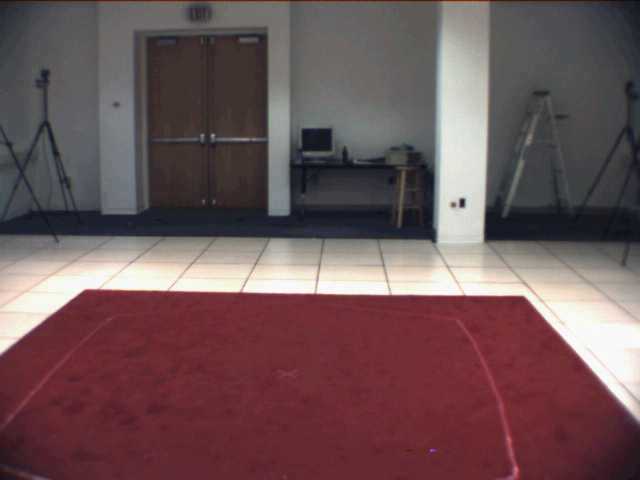
\includegraphics[width=0.31\textwidth]{bk_C1}}
  \subcaptionbox{C2}{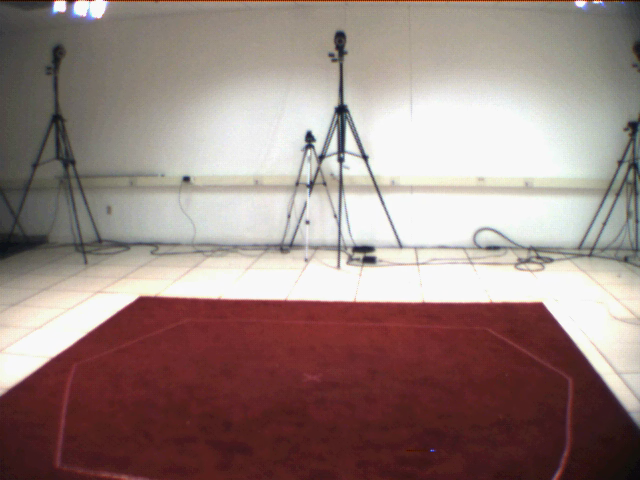
\includegraphics[width=0.31\textwidth]{bk_C2}}
  \subcaptionbox{C3}{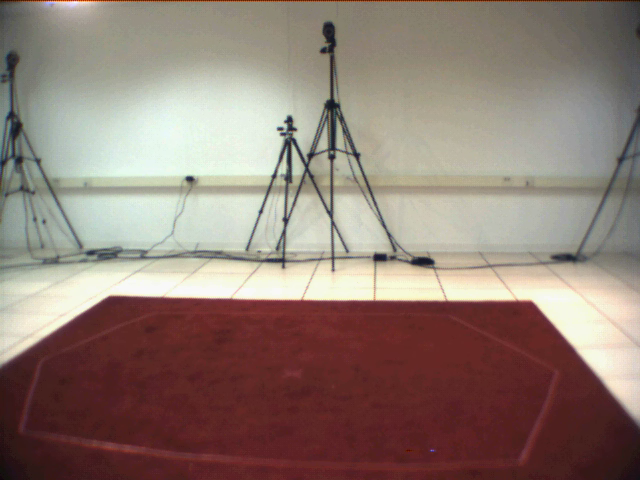
\includegraphics[width=0.31\textwidth]{bk_C3}}
  \caption{HumanEva背景}\label{fig:background}
\end{figure}
\subsection{计算背景数据}
给出的背景不是单张图片,而是一段视频,因此可利用的信息更多。本文假定视频中的$N$帧图像每个像素点都满足高斯分布,记像素点$\mathbf{c}=(r,g,b)$,则$\mathbf{c}\sim \mathcal{N}(\mu,\sigma)$,通过统计所有视频帧可以算出$\mu$和$\sigma$,用待分割图片中的每一个像素点代入高斯分布,即可算出该点是否为背景的概率。给定一个阈值,即可产生一个粗糙的二值图分割,见图\ref{fig:bk1}。
\begin{figure}[htbp]
  \centering
  \subcaptionbox{原图}{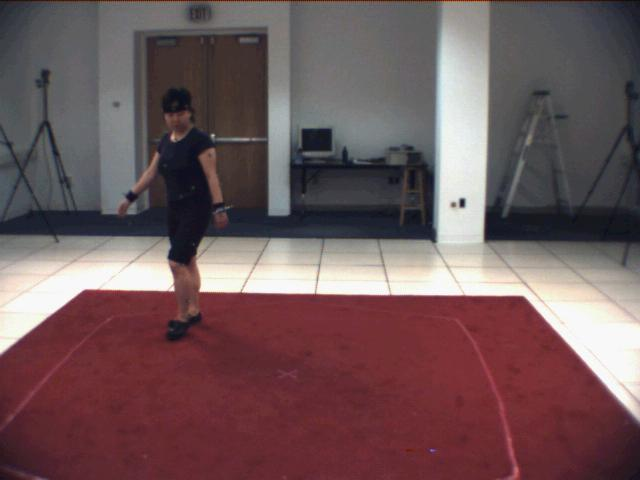
\includegraphics[width=0.45\textwidth]{bkimage}\hspace{.5cm}}
  \subcaptionbox{背景概率分割}{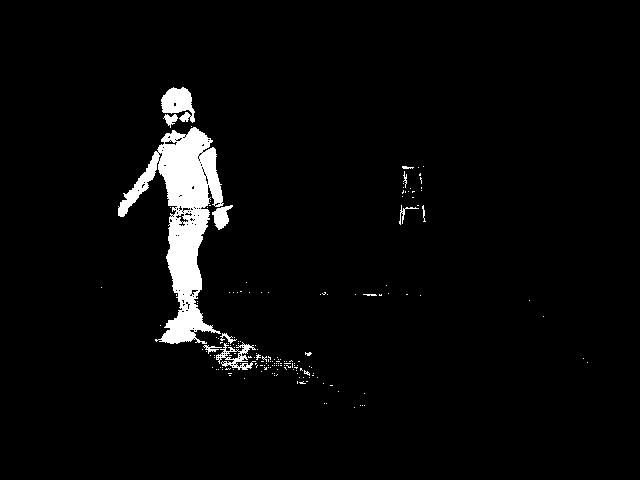
\includegraphics[width=0.45\textwidth]{bk1}}
  \caption{HumanEva背景分割1}\label{fig:bk1}
\end{figure}

\subsection{局部优化}
可以看出,用简单的阈值分割无法保证正确性,部分背景被认为是前景(即所需人物),而前景中夹杂的与背景相似的颜色则被认为是背景,于是又做了很多优化。首先,需要去掉人物产生的阴影。%所用方法
阴影去除后的效果见图\ref{fig:bk2foot}。

\begin{figure}[htbp]
  \centering
  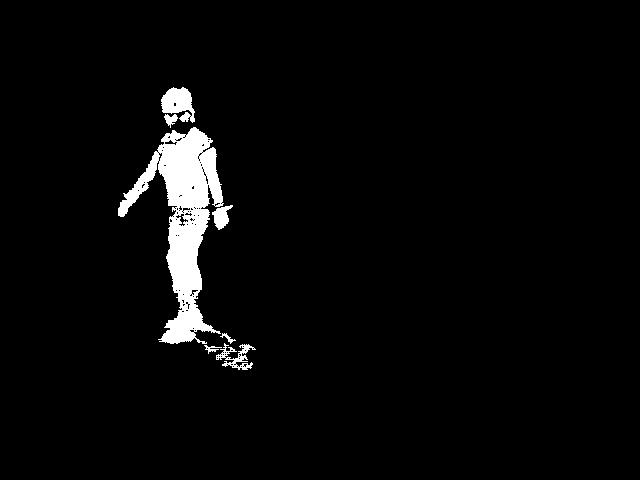
\includegraphics[width=0.45\textwidth]{bk3}
  \caption{HumanEva背景分割2}\label{fig:bk2foot}
\end{figure}

此时还有一些背景噪音,接着去掉了前景中面积较小的部分,面积的阈值可以选的小一些,在这里选择为40像素(图像为$480\times 640$像素),这些部分大多都是未能剔除的环境噪音,此时结果参见图\ref{fig:bk3small},然而还有大块背景未能去掉,这时,先找到图中最大面积区域的位置,该区域被近似为前景位置,将偏离该点较远的区域都认为是背景(因为数据库中人物的动作范围不大,长宽均有限,这里把阈值选为80 像素),可以从图\ref{fig:bk3far}看出偏远大块的背景已经被去掉。

\begin{figure}[htbp]
  \centering
  \subcaptionbox{去掉小块背景\label{fig:bk3small}}{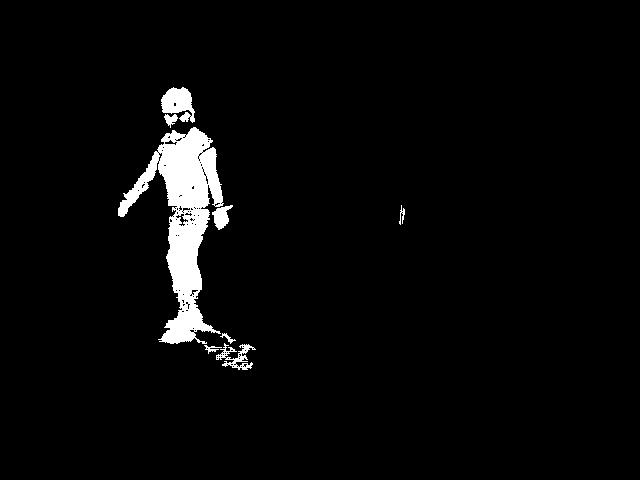
\includegraphics[width=0.45\textwidth]{bk2}}
  \subcaptionbox{去掉偏远背景\label{fig:bk3far}}{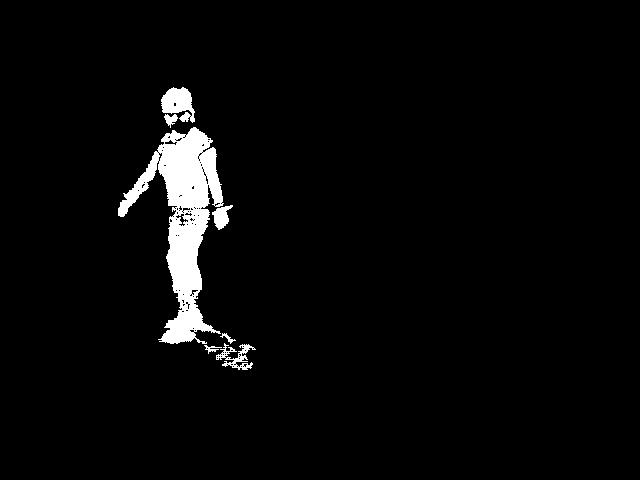
\includegraphics[width=0.45\textwidth]{bk3}}
  \caption{HumanEva背景分割3}
\end{figure}

由于人物的脸部等地方有较大缺失,于是接着做了8次膨胀(半径为1的圆形,见图\ref{fig:bk4dilate}),和8次腐蚀(同样半径为1,见图\ref{fig:bk4erode}),最后做一次背景抹除(面积小于400像素的都被消去),此时只剩下了单一连通的前景。

\begin{figure}[htbp]
  \centering
  \subcaptionbox{膨胀\label{fig:bk4dilate}}{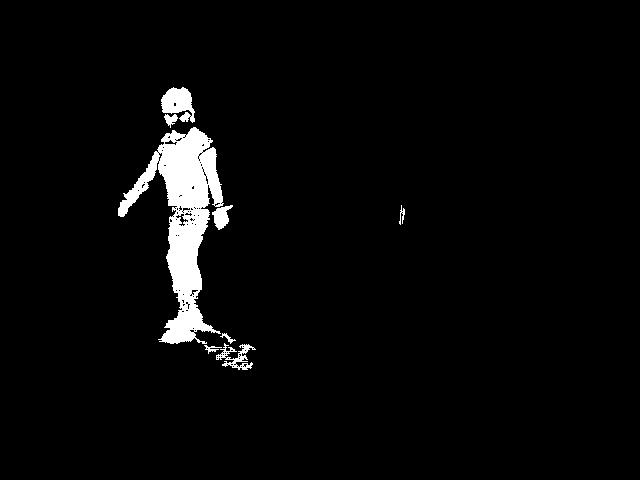
\includegraphics[width=0.45\textwidth]{bk2}}
  \subcaptionbox{腐蚀\label{fig:bk4erode}}{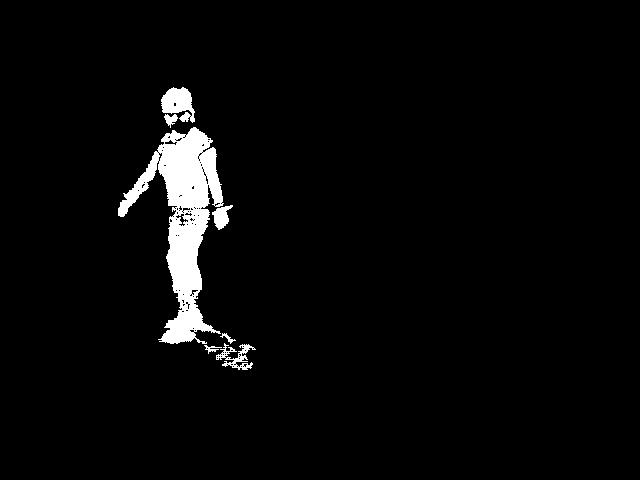
\includegraphics[width=0.45\textwidth]{bk3}}
  \caption{HumanEva背景分割4}
\end{figure}

与\cite{Poppe2007}对比可以看出,该文献的前景(见图\ref{fig:bk_cmp_org})有较多空洞,这对于HoG的计算会带来很大误差,而本文提出的分割方法(见图\ref{fig:bk_cmp_my})没有小块噪音,整个前景连为一体,虽然在边缘轮廓不是特别准确,但是对于HoG特征来说影响不大。

\begin{figure}[htbp]
  \centering
  \subcaptionbox{Poppe等人分割结果\label{fig:bk_cmp_org}}{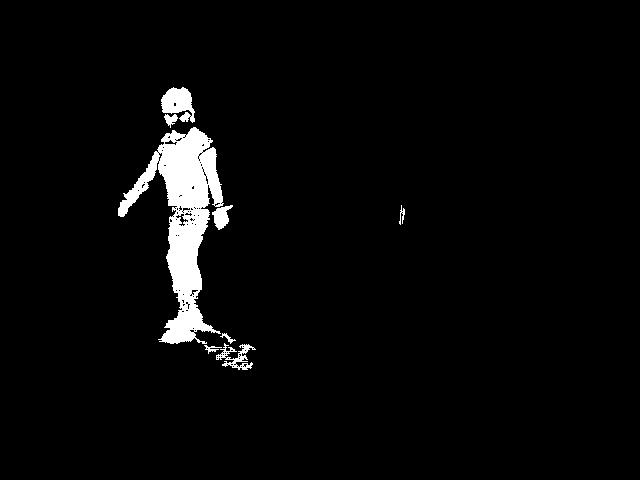
\includegraphics[width=0.45\textwidth]{bk2}}
  \subcaptionbox{本文结果\label{fig:bk_cmp_my}}{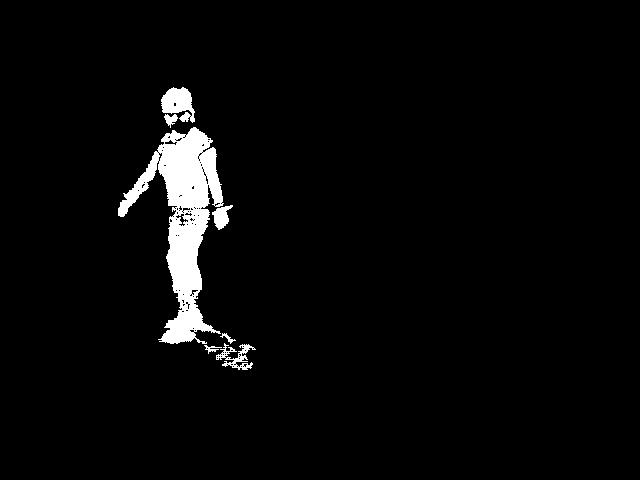
\includegraphics[width=0.45\textwidth]{bk3}}
  \caption{背景分割对比}
\end{figure}

此外,在处理演员2和3的时候由于衣服颜色和背景过于相像,出现了图\ref{fig:bkerr} 所示的错误,针对这种特殊情况,先找到前景所占矩形区域,然后填充矩形区域中上部60\%范围内的空洞。这一操作虽然不至于填充两腿缝隙,但对于胳膊与腰造成的空洞也会一并填充,鉴于这种情况出现的帧数极少,故忽略此问题。

\begin{figure}[htbp]
  \centering
  \subcaptionbox{错误1}{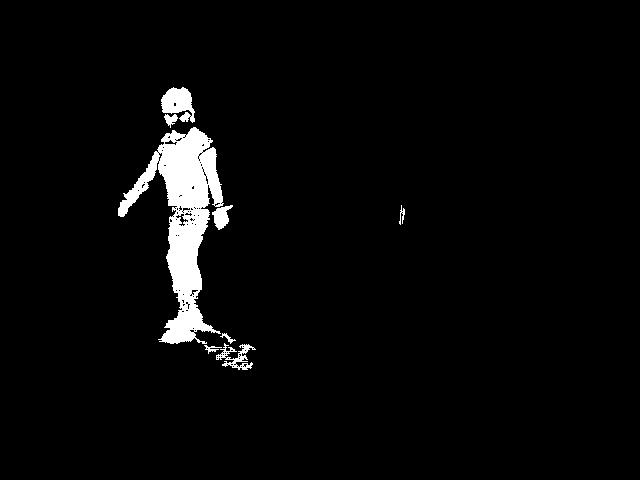
\includegraphics[width=0.45\textwidth]{bk2}}
  \subcaptionbox{错误2}{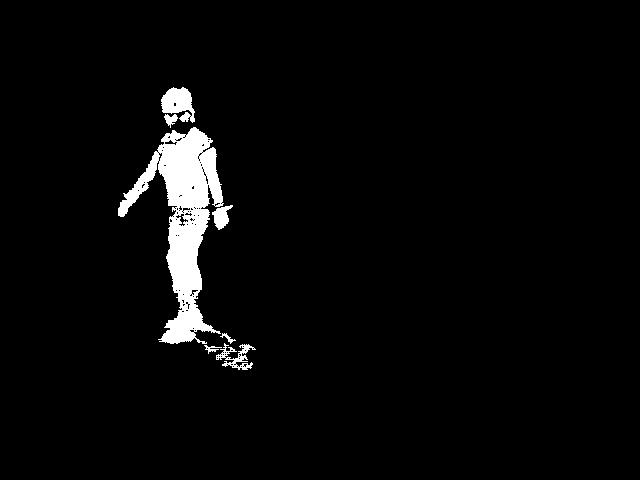
\includegraphics[width=0.45\textwidth]{bk3}}
  \caption{背景分割错误}\label{fig:bkerr}
\end{figure}

\section{HOG特征}
\subsection{概述}
HOG特征最早由Navneet Dalal和Bill Triggs在2005年提出~\cite{Dalal05histogramsof},被成功地用于目标检测,尤其是行人检测。该方法是对图像的局部区域出现的方向梯度进行统计,和SIFT(scale-invariant feature transform)相似,不同的是HOG用了重叠的局部对比度归一化(overlapping local contrast normalization)技术。HOG描述子的主要贡献是很好地描述了局部区域的边缘方向密度。对图像进行归一化后,能够很好地保证照射和阴影不变性。与其他方法相比,HOG有很好的几何和光学转化不变性,因此十分适合行人检测和姿态估计。
\subsection{计算HOG描述子}
HOG特征的提取方法主要步骤如下:
\begin{enumerate}
  \item 转化为灰度图像
  \item 划分成若干子区域(cell)
  \item 计算每个像素的梯度
  \item 统计每个子区域内梯度直方图
\end{enumerate}

具体说来,本文将$r,g,b$三个通道认为是三张灰度图,分别求取HOG特征,最后取每一维最大值,最后做归一化处理。伪代码见代码\ref{alg:maxhog}。

\begin{algorithm}
  \caption{MAX-HOG}\label{alg:maxhog}
  \begin{algorithmic}[1]
    %\PROCEDURE {MAX-HOG}{$image$}
    \FOR{$i=0$ to $image.NumberOfChannels$}
        \STATE H($i$) $\leftarrow$ GetHOG($image.channel(i)$)
    \ENDFOR
    
      H $\leftarrow$ MAX(H($i$))\\
      H $\leftarrow$ L1Norm(H)\\
    \RETURN H
  \end{algorithmic}
\end{algorithm}

\section{皮肤特征}
由于人的皮肤是一个不变的特征,而且胳膊、头的位置对于姿态估计有重要作用,因此充分利用皮肤特征是十分必要的。对于姿态估计,我们只关心胳膊、头的位置,因此本文用位置、面积信息来描述皮肤特征。首先,需要判断每个像素属于皮肤的概率,为了简化问题,本文假定皮肤颜色在YCbCr空间服从高斯分布,均值和方差均为手工给出。由于人们往往是穿着长裤,因此只能检测到头和左右臂这三个部分,而在穿长袖衣服时则只能检测到头和左右手。因此本文只选取概率最大的三个区域\footnote{只考虑ROI中的上半部分。有时候会小于三个区域,因为手和头部相连。},分别认为是头、左臂和右臂。按面积由大到小排序,每一个区域用$\mathbf{r}=(x,y,s)$表示,$(x,y)$为区域的重心坐标,$s$为区域面积。
\begin{figure}[htbp]
  \centering
  \subcaptionbox{原图}{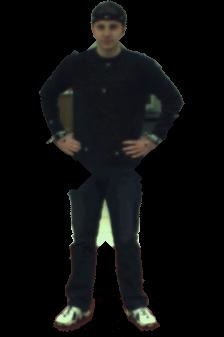
\includegraphics[width=0.3\textwidth]{skin}\hspace{1cm}}
  \subcaptionbox{皮肤检测}{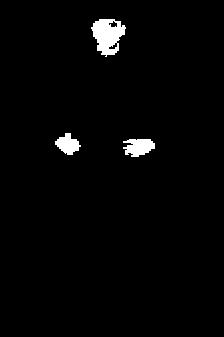
\includegraphics[width=0.3\textwidth]{skinbw}}
  \caption{皮肤检测}
\end{figure}

\section{特征表示}
\label{sec:feature}

